% Options for packages loaded elsewhere
\PassOptionsToPackage{unicode}{hyperref}
\PassOptionsToPackage{hyphens}{url}
\PassOptionsToPackage{dvipsnames,svgnames,x11names}{xcolor}
%
\documentclass[
  letterpaper,
  DIV=11,
  numbers=noendperiod]{scrartcl}

\usepackage{amsmath,amssymb}
\usepackage{lmodern}
\usepackage{iftex}
\ifPDFTeX
  \usepackage[T1]{fontenc}
  \usepackage[utf8]{inputenc}
  \usepackage{textcomp} % provide euro and other symbols
\else % if luatex or xetex
  \usepackage{unicode-math}
  \defaultfontfeatures{Scale=MatchLowercase}
  \defaultfontfeatures[\rmfamily]{Ligatures=TeX,Scale=1}
\fi
% Use upquote if available, for straight quotes in verbatim environments
\IfFileExists{upquote.sty}{\usepackage{upquote}}{}
\IfFileExists{microtype.sty}{% use microtype if available
  \usepackage[]{microtype}
  \UseMicrotypeSet[protrusion]{basicmath} % disable protrusion for tt fonts
}{}
\makeatletter
\@ifundefined{KOMAClassName}{% if non-KOMA class
  \IfFileExists{parskip.sty}{%
    \usepackage{parskip}
  }{% else
    \setlength{\parindent}{0pt}
    \setlength{\parskip}{6pt plus 2pt minus 1pt}}
}{% if KOMA class
  \KOMAoptions{parskip=half}}
\makeatother
\usepackage{xcolor}
\setlength{\emergencystretch}{3em} % prevent overfull lines
\setcounter{secnumdepth}{5}
% Make \paragraph and \subparagraph free-standing
\ifx\paragraph\undefined\else
  \let\oldparagraph\paragraph
  \renewcommand{\paragraph}[1]{\oldparagraph{#1}\mbox{}}
\fi
\ifx\subparagraph\undefined\else
  \let\oldsubparagraph\subparagraph
  \renewcommand{\subparagraph}[1]{\oldsubparagraph{#1}\mbox{}}
\fi

\usepackage{color}
\usepackage{fancyvrb}
\newcommand{\VerbBar}{|}
\newcommand{\VERB}{\Verb[commandchars=\\\{\}]}
\DefineVerbatimEnvironment{Highlighting}{Verbatim}{commandchars=\\\{\}}
% Add ',fontsize=\small' for more characters per line
\usepackage{framed}
\definecolor{shadecolor}{RGB}{241,243,245}
\newenvironment{Shaded}{\begin{snugshade}}{\end{snugshade}}
\newcommand{\AlertTok}[1]{\textcolor[rgb]{0.68,0.00,0.00}{#1}}
\newcommand{\AnnotationTok}[1]{\textcolor[rgb]{0.37,0.37,0.37}{#1}}
\newcommand{\AttributeTok}[1]{\textcolor[rgb]{0.40,0.45,0.13}{#1}}
\newcommand{\BaseNTok}[1]{\textcolor[rgb]{0.68,0.00,0.00}{#1}}
\newcommand{\BuiltInTok}[1]{\textcolor[rgb]{0.00,0.23,0.31}{#1}}
\newcommand{\CharTok}[1]{\textcolor[rgb]{0.13,0.47,0.30}{#1}}
\newcommand{\CommentTok}[1]{\textcolor[rgb]{0.37,0.37,0.37}{#1}}
\newcommand{\CommentVarTok}[1]{\textcolor[rgb]{0.37,0.37,0.37}{\textit{#1}}}
\newcommand{\ConstantTok}[1]{\textcolor[rgb]{0.56,0.35,0.01}{#1}}
\newcommand{\ControlFlowTok}[1]{\textcolor[rgb]{0.00,0.23,0.31}{#1}}
\newcommand{\DataTypeTok}[1]{\textcolor[rgb]{0.68,0.00,0.00}{#1}}
\newcommand{\DecValTok}[1]{\textcolor[rgb]{0.68,0.00,0.00}{#1}}
\newcommand{\DocumentationTok}[1]{\textcolor[rgb]{0.37,0.37,0.37}{\textit{#1}}}
\newcommand{\ErrorTok}[1]{\textcolor[rgb]{0.68,0.00,0.00}{#1}}
\newcommand{\ExtensionTok}[1]{\textcolor[rgb]{0.00,0.23,0.31}{#1}}
\newcommand{\FloatTok}[1]{\textcolor[rgb]{0.68,0.00,0.00}{#1}}
\newcommand{\FunctionTok}[1]{\textcolor[rgb]{0.28,0.35,0.67}{#1}}
\newcommand{\ImportTok}[1]{\textcolor[rgb]{0.00,0.46,0.62}{#1}}
\newcommand{\InformationTok}[1]{\textcolor[rgb]{0.37,0.37,0.37}{#1}}
\newcommand{\KeywordTok}[1]{\textcolor[rgb]{0.00,0.23,0.31}{#1}}
\newcommand{\NormalTok}[1]{\textcolor[rgb]{0.00,0.23,0.31}{#1}}
\newcommand{\OperatorTok}[1]{\textcolor[rgb]{0.37,0.37,0.37}{#1}}
\newcommand{\OtherTok}[1]{\textcolor[rgb]{0.00,0.23,0.31}{#1}}
\newcommand{\PreprocessorTok}[1]{\textcolor[rgb]{0.68,0.00,0.00}{#1}}
\newcommand{\RegionMarkerTok}[1]{\textcolor[rgb]{0.00,0.23,0.31}{#1}}
\newcommand{\SpecialCharTok}[1]{\textcolor[rgb]{0.37,0.37,0.37}{#1}}
\newcommand{\SpecialStringTok}[1]{\textcolor[rgb]{0.13,0.47,0.30}{#1}}
\newcommand{\StringTok}[1]{\textcolor[rgb]{0.13,0.47,0.30}{#1}}
\newcommand{\VariableTok}[1]{\textcolor[rgb]{0.07,0.07,0.07}{#1}}
\newcommand{\VerbatimStringTok}[1]{\textcolor[rgb]{0.13,0.47,0.30}{#1}}
\newcommand{\WarningTok}[1]{\textcolor[rgb]{0.37,0.37,0.37}{\textit{#1}}}

\providecommand{\tightlist}{%
  \setlength{\itemsep}{0pt}\setlength{\parskip}{0pt}}\usepackage{longtable,booktabs,array}
\usepackage{calc} % for calculating minipage widths
% Correct order of tables after \paragraph or \subparagraph
\usepackage{etoolbox}
\makeatletter
\patchcmd\longtable{\par}{\if@noskipsec\mbox{}\fi\par}{}{}
\makeatother
% Allow footnotes in longtable head/foot
\IfFileExists{footnotehyper.sty}{\usepackage{footnotehyper}}{\usepackage{footnote}}
\makesavenoteenv{longtable}
\usepackage{graphicx}
\makeatletter
\def\maxwidth{\ifdim\Gin@nat@width>\linewidth\linewidth\else\Gin@nat@width\fi}
\def\maxheight{\ifdim\Gin@nat@height>\textheight\textheight\else\Gin@nat@height\fi}
\makeatother
% Scale images if necessary, so that they will not overflow the page
% margins by default, and it is still possible to overwrite the defaults
% using explicit options in \includegraphics[width, height, ...]{}
\setkeys{Gin}{width=\maxwidth,height=\maxheight,keepaspectratio}
% Set default figure placement to htbp
\makeatletter
\def\fps@figure{htbp}
\makeatother
\newlength{\cslhangindent}
\setlength{\cslhangindent}{1.5em}
\newlength{\csllabelwidth}
\setlength{\csllabelwidth}{3em}
\newlength{\cslentryspacingunit} % times entry-spacing
\setlength{\cslentryspacingunit}{\parskip}
\newenvironment{CSLReferences}[2] % #1 hanging-ident, #2 entry spacing
 {% don't indent paragraphs
  \setlength{\parindent}{0pt}
  % turn on hanging indent if param 1 is 1
  \ifodd #1
  \let\oldpar\par
  \def\par{\hangindent=\cslhangindent\oldpar}
  \fi
  % set entry spacing
  \setlength{\parskip}{#2\cslentryspacingunit}
 }%
 {}
\usepackage{calc}
\newcommand{\CSLBlock}[1]{#1\hfill\break}
\newcommand{\CSLLeftMargin}[1]{\parbox[t]{\csllabelwidth}{#1}}
\newcommand{\CSLRightInline}[1]{\parbox[t]{\linewidth - \csllabelwidth}{#1}\break}
\newcommand{\CSLIndent}[1]{\hspace{\cslhangindent}#1}

\usepackage{booktabs}
\usepackage{longtable}
\usepackage{array}
\usepackage{multirow}
\usepackage{wrapfig}
\usepackage{float}
\usepackage{colortbl}
\usepackage{pdflscape}
\usepackage{tabu}
\usepackage{threeparttable}
\usepackage{threeparttablex}
\usepackage[normalem]{ulem}
\usepackage{makecell}
\usepackage{xcolor}
\KOMAoption{captions}{tableheading}
\makeatletter
\makeatother
\makeatletter
\makeatother
\makeatletter
\@ifpackageloaded{caption}{}{\usepackage{caption}}
\AtBeginDocument{%
\ifdefined\contentsname
  \renewcommand*\contentsname{Table of contents}
\else
  \newcommand\contentsname{Table of contents}
\fi
\ifdefined\listfigurename
  \renewcommand*\listfigurename{List of Figures}
\else
  \newcommand\listfigurename{List of Figures}
\fi
\ifdefined\listtablename
  \renewcommand*\listtablename{List of Tables}
\else
  \newcommand\listtablename{List of Tables}
\fi
\ifdefined\figurename
  \renewcommand*\figurename{Figure}
\else
  \newcommand\figurename{Figure}
\fi
\ifdefined\tablename
  \renewcommand*\tablename{Table}
\else
  \newcommand\tablename{Table}
\fi
}
\@ifpackageloaded{float}{}{\usepackage{float}}
\floatstyle{ruled}
\@ifundefined{c@chapter}{\newfloat{codelisting}{h}{lop}}{\newfloat{codelisting}{h}{lop}[chapter]}
\floatname{codelisting}{Listing}
\newcommand*\listoflistings{\listof{codelisting}{List of Listings}}
\makeatother
\makeatletter
\@ifpackageloaded{caption}{}{\usepackage{caption}}
\@ifpackageloaded{subcaption}{}{\usepackage{subcaption}}
\makeatother
\makeatletter
\@ifpackageloaded{tcolorbox}{}{\usepackage[many]{tcolorbox}}
\makeatother
\makeatletter
\@ifundefined{shadecolor}{\definecolor{shadecolor}{rgb}{.97, .97, .97}}
\makeatother
\makeatletter
\makeatother
\ifLuaTeX
  \usepackage{selnolig}  % disable illegal ligatures
\fi
\IfFileExists{bookmark.sty}{\usepackage{bookmark}}{\usepackage{hyperref}}
\IfFileExists{xurl.sty}{\usepackage{xurl}}{} % add URL line breaks if available
\urlstyle{same} % disable monospaced font for URLs
\hypersetup{
  pdftitle={Sample Paper},
  pdfauthor={Sample Student},
  colorlinks=true,
  linkcolor={blue},
  filecolor={Maroon},
  citecolor={Blue},
  urlcolor={Blue},
  pdfcreator={LaTeX via pandoc}}

\title{Sample Paper}
\author{Sample Student}
\date{}

\begin{document}
\maketitle
\begin{abstract}
This is a sample abstract for the sample paper just to show how you can
add an abstract.
\end{abstract}
\ifdefined\Shaded\renewenvironment{Shaded}{\begin{tcolorbox}[interior hidden, borderline west={3pt}{0pt}{shadecolor}, frame hidden, boxrule=0pt, sharp corners, enhanced, breakable]}{\end{tcolorbox}}\fi

\renewcommand*\contentsname{Table of contents}
{
\hypersetup{linkcolor=}
\setcounter{tocdepth}{3}
\tableofcontents
}
\listoffigures
\listoftables
\hypertarget{introduction}{%
\section{Introduction}\label{introduction}}

In this sample paper a few tables, plots and pieces of text are
reproduced from the register analysis case study. The goal is to
illustrate some things to be expected from a final paper from this
course.

For example, a key aspect of the corpus in this analysis is its register
structure. Therefore, next to a brief description of the corpus itself,
it would make sense to add and describe a table such as
Table~\ref{tbl-registers}.

\hypertarget{tbl-registers}{}
\begin{table}
\caption{\label{tbl-registers}List of components of the Brown corpus with the registers they
represent, number of files and number of tokens. }\tabularnewline

\centering
\begin{tabular}[t]{l|r|l|r|r}
\hline
Section & Component & Register & Files & Tokens\\
\hline
 & a & Press-reportage & 44 & 100 554\\
\cline{2-5}
 & b & Press-editorial & 27 & 61 604\\
\cline{2-5}
 & c & Press-reviews & 17 & 40 704\\
\cline{2-5}
 & d & Religion & 17 & 39 399\\
\cline{2-5}
 & e & Skills \& hobbies & 36 & 82 345\\
\cline{2-5}
 & f & Popular Lore & 48 & 110 299\\
\cline{2-5}
 & g & Belles Lettres, Biography, Memoirs, etc. & 75 & 173 096\\
\cline{2-5}
 & h & Miscellaneous & 30 & 70 117\\
\cline{2-5}
\multirow{-9}{*}{\raggedright\arraybackslash Informative} & j & Learned & 80 & 181 888\\
\cline{1-5}
 & k & General Fiction & 29 & 68 488\\
\cline{2-5}
 & l & Mystery and Detective Fiction & 24 & 57 169\\
\cline{2-5}
 & m & Science Fiction & 6 & 14 470\\
\cline{2-5}
 & n & Adventure and Western Fiction & 29 & 69 342\\
\cline{2-5}
 & p & Romance and Love Stories & 29 & 70 022\\
\cline{2-5}
\multirow{-6}{*}{\raggedright\arraybackslash Imaginative} & r & Humor & 9 & 21 695\\
\hline
\end{tabular}
\end{table}

Tables can be written either in R chunks or manually, but in any case
they should have a caption and be cross-referenceable, like
Table~\ref{tbl-pos}. That table defines the 13 numerical variables,
which are very few compared to what Biber (1988) used.

\hypertarget{tbl-pos}{}
\begin{longtable}[]{@{}
  >{\raggedright\arraybackslash}p{(\columnwidth - 2\tabcolsep) * \real{0.2000}}
  >{\raggedright\arraybackslash}p{(\columnwidth - 2\tabcolsep) * \real{0.8000}}@{}}
\caption{\label{tbl-pos}Numerical variables and their
definitions:}\tabularnewline
\toprule()
\begin{minipage}[b]{\linewidth}\raggedright
Name
\end{minipage} & \begin{minipage}[b]{\linewidth}\raggedright
Value
\end{minipage} \\
\midrule()
\endfirsthead
\toprule()
\begin{minipage}[b]{\linewidth}\raggedright
Name
\end{minipage} & \begin{minipage}[b]{\linewidth}\raggedright
Value
\end{minipage} \\
\midrule()
\endhead
\texttt{ttr} & Type token ratio (number of types divided by number of
tokens)\footnote{The type token ratio of different texts can only be
  compared if they have similar lengths, which is the case with the
  Brown corpus.} \\
\texttt{word\_len} & Average word length, in characters \\
\texttt{p\_mw} & Proportion of combined tags; typically clitics as in
\emph{she's} \\
\texttt{p\_c} & Proportion of punctuation characters \\
\texttt{p\_ppss} & Proportion of personal pronouns nominative, besides
third person singular \\
\texttt{p\_noun} & Proportion of nouns \\
\texttt{p\_bigr} & Number of unique word bigrams, relative to document
size \\
\texttt{p\_nomin} & Proportion of nominalisations (nouns ending in
\emph{-tion}, \emph{-ment}, \emph{-ness}, or \emph{-ity}) \\
\texttt{p\_pobi} & Number of unique pos tag bigrams, relative to
document size \\
\texttt{p\_adj} & Proportion of adjectives \\
\texttt{p\_neg} & Number of negations, relative to document size \\
\texttt{p\_adv} & Proportion of adverbs \\
\texttt{p\_qual} & Number of qualifiers, relative to document size \\
\bottomrule()
\end{longtable}

The annotation was performed with the help of the
\texttt{\{tidyverse\}}, \texttt{\{mclm\}} and \texttt{\{xml2\}} packages
(Wickham et al. 2019; Speelman \& Montes 2022; Wickham, Hester \& Ooms
2021). Yes, packages should be cited as well.

\hypertarget{intermediate-session}{%
\section{Intermediate session}\label{intermediate-session}}

For specific code ran that is key to the paper, it might be interesting
to show it (without evaluating) it in the paper, for example:

\begin{Shaded}
\begin{Highlighting}[]
\NormalTok{dataset }\OtherTok{\textless{}{-}} \FunctionTok{read\_tsv}\NormalTok{(}\FunctionTok{here}\NormalTok{(}\StringTok{"register{-}analysis.tsv"}\NormalTok{), }\AttributeTok{show\_col\_types =} \ConstantTok{FALSE}\NormalTok{)}
\NormalTok{fa }\OtherTok{\textless{}{-}}\NormalTok{ dataset }\SpecialCharTok{\%\textgreater{}\%} \FunctionTok{data.frame}\NormalTok{(}\AttributeTok{row.names =} \StringTok{"filename"}\NormalTok{) }\SpecialCharTok{\%\textgreater{}\%} 
  \FunctionTok{as.matrix}\NormalTok{() }\SpecialCharTok{\%\textgreater{}\%} \FunctionTok{factanal}\NormalTok{(}\AttributeTok{factors =} \DecValTok{4}\NormalTok{, }\AttributeTok{scores =} \StringTok{"regression"}\NormalTok{)}
\end{Highlighting}
\end{Shaded}

But, given that the code is also shared, it is not strictly necessary.
We might want to add more references, though, such as citing R Core Team
(2022), adding Levshina (2015) to Biber (1988), and including a quote:

\begin{quote}
In the description of textual variation, where the factors represent
underlying textual dimensions, there is no reason to assume that the
factors are completely uncorrelated, and therefore a Promax rotation is
recommended. (Biber 1988: 85)
\end{quote}

Of course, we should use cross references to refer to useful figures and
tables such as Figure~\ref{fig-scores} and Table~\ref{tbl-factors}.

\hypertarget{tbl-factors}{}
\begin{table}
\caption{\label{tbl-factors}Loadings of the four factors. }\tabularnewline

\centering\begingroup\fontsize{22}{24}\selectfont

\begin{tabular}[t]{l|r|r|r|r}
\hline
Variable & Factor1 & Factor2 & Factor3 & Factor4\\
\hline
ttr &  &  & 0.98 & \\
\hline
word\_len & 0.88 & -0.35 &  & \\
\hline
p\_bigr &  &  & 0.92 & \\
\hline
p\_pobi & -0.35 &  & 0.42 & 0.62\\
\hline
p\_mw &  & 0.95 &  & \\
\hline
p\_c & -0.40 & 0.54 &  & \\
\hline
p\_nomin & 0.79 &  &  & \\
\hline
p\_noun & 0.61 & -0.39 &  & -0.47\\
\hline
p\_ppss & -0.44 & 0.53 &  & 0.31\\
\hline
p\_adj & 0.68 & -0.30 &  & \\
\hline
p\_neg &  & 0.87 &  & \\
\hline
p\_adv & -0.38 & 0.33 &  & 0.58\\
\hline
p\_qual &  &  &  & 0.67\\
\hline
\end{tabular}
\endgroup{}
\end{table}

\begin{figure}

{\centering 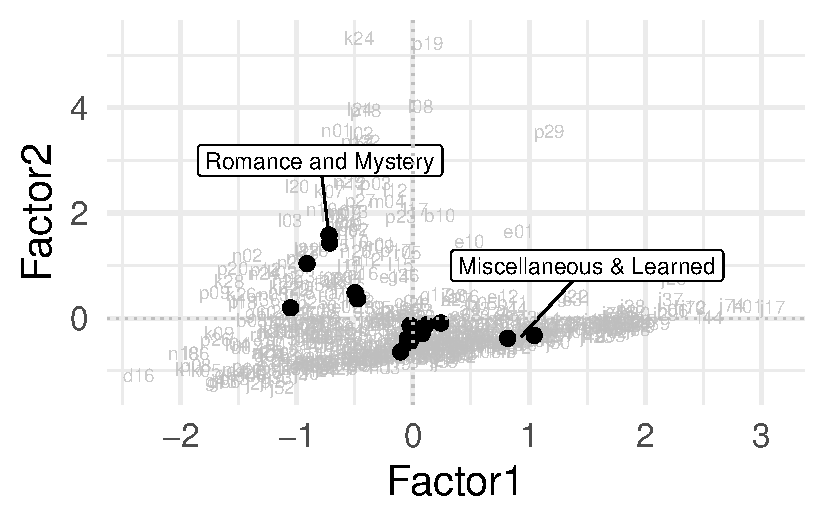
\includegraphics{sample-paper_files/figure-pdf/fig-scores-1.pdf}

}

\caption{\label{fig-scores}Scatterplot of document scores with the first
two factors as dimensions and relevant registers annotated.}

\end{figure}

\hypertarget{discussion-of-results}{%
\section{Discussion of results}\label{discussion-of-results}}

More plots and tables would probably be in order, this is just a sample!
But it will also be useful to add linguistic examples, such as (1),
maybe with interlinear glosses using \texttt{\{glossr\}}!

\begin{enumerate}
\def\labelenumi{(\arabic{enumi})}
\tightlist
\item
  He who has not the Son has not the life .
\end{enumerate}

\hypertarget{conclusion}{%
\section{Conclusion}\label{conclusion}}

In conclusion, best of luck to everyone!

\hypertarget{refs}{}
\begin{CSLReferences}{1}{0}
\leavevmode\vadjust pre{\hypertarget{ref-biber_1988}{}}%
Biber, Douglas. 1988. \emph{Variation across {Speech} and {Writing}}.
First. {Cambridge University Press}.
\url{https://doi.org/10.1017/CBO9780511621024}.

\leavevmode\vadjust pre{\hypertarget{ref-levshina_2015}{}}%
Levshina, Natalia. 2015. \emph{How to do linguistics with {R}: Data
exploration and statistical analysis}. {Amsterdam; Philadelphia}: {John
Benjamins Publishing Company}.

\leavevmode\vadjust pre{\hypertarget{ref-R-base}{}}%
R Core Team. 2022. \emph{R: A language and environment for statistical
computing}. Vienna, Austria: R Foundation for Statistical Computing.
\url{https://www.R-project.org/}.

\leavevmode\vadjust pre{\hypertarget{ref-R-mclm}{}}%
Speelman, Dirk \& Mariana Montes. 2022. \emph{Mclm: Mastering corpus
linguistics methods}. \url{https://CRAN.R-project.org/package=mclm}.

\leavevmode\vadjust pre{\hypertarget{ref-tidyverse2019}{}}%
Wickham, Hadley, Mara Averick, Jennifer Bryan, Winston Chang, Lucy
D'Agostino McGowan, Romain François, Garrett Grolemund, et al. 2019.
Welcome to the {tidyverse}. \emph{Journal of Open Source Software}
4(43). 1686. \url{https://doi.org/10.21105/joss.01686}.

\leavevmode\vadjust pre{\hypertarget{ref-R-xml2}{}}%
Wickham, Hadley, Jim Hester \& Jeroen Ooms. 2021. \emph{xml2: Parse
XML}. \url{https://CRAN.R-project.org/package=xml2}.

\end{CSLReferences}



\end{document}
